\documentclass[11pt]{article}
\usepackage[margin=1in]{geometry}
\usepackage{amsmath,amssymb,amsthm,mathtools}
\usepackage{graphicx}
\usepackage{microtype}
\usepackage[hidelinks]{hyperref}
\newtheorem{theorem}{Theorem}
\newtheorem{lemma}[theorem]{Lemma}
\newtheorem{corollary}[theorem]{Corollary}
\newcommand{\Cu}{C_u^*}
\newcommand{\ellTwo}{\ell_2}
\newcommand{\SOT}{\mathop{\mathrm{SOT}\!-\!\sum}}
\title{Bounded-rank block projections and bounded-rank subsequences admit rank-one selections}
\author{Automated Math Discovery Run \texttt{fa\_banach\_001}\\Model: GPT5.6}
\date{22 July 2026}
\begin{document}
\maketitle
\begin{center}
\fbox{\begin{minipage}{0.91\textwidth}
\textbf{Claimed status: substantial partial result, subject to human review.}
The results settle all uniformly bounded-rank block families and the
infinite-subsequence question whenever one finite rank occurs infinitely
often.  The unbounded-rank and infinite-rank cases of Question~6.1 remain.
\end{minipage}}
\end{center}
\section{Source questions}
Braga, Farah, and Vignati ask in Question~6.1 whether a sequence of
projections $p_n\in\Cu(X)$ whose every strong subseries belongs to
$\Cu(X)$ admits rank-one subprojections with the same property
\cite[Question~6.1, p.~20]{BFV}. The exact source passage is reproduced below.
\begin{figure}[ht]
\centering

\includegraphics[width=0.95\textwidth]{figures/open_problem_crop.png}
\caption{Question~6.1 in the source paper.}
\end{figure}
The rank-two block case was restated as an explicit open question in
Vignati's 2026 habilitation \cite[Question~5.31, p.~53]{Vig}: if
$p=\SOT_n p_n$ is a noncompact block ghost projection and every $p_n$
has rank two, must there be rank-one $q_n\leq p_n$ such that
$\SOT_nq_n\in\Cu(X)$?
\begin{figure}[ht]
\centering
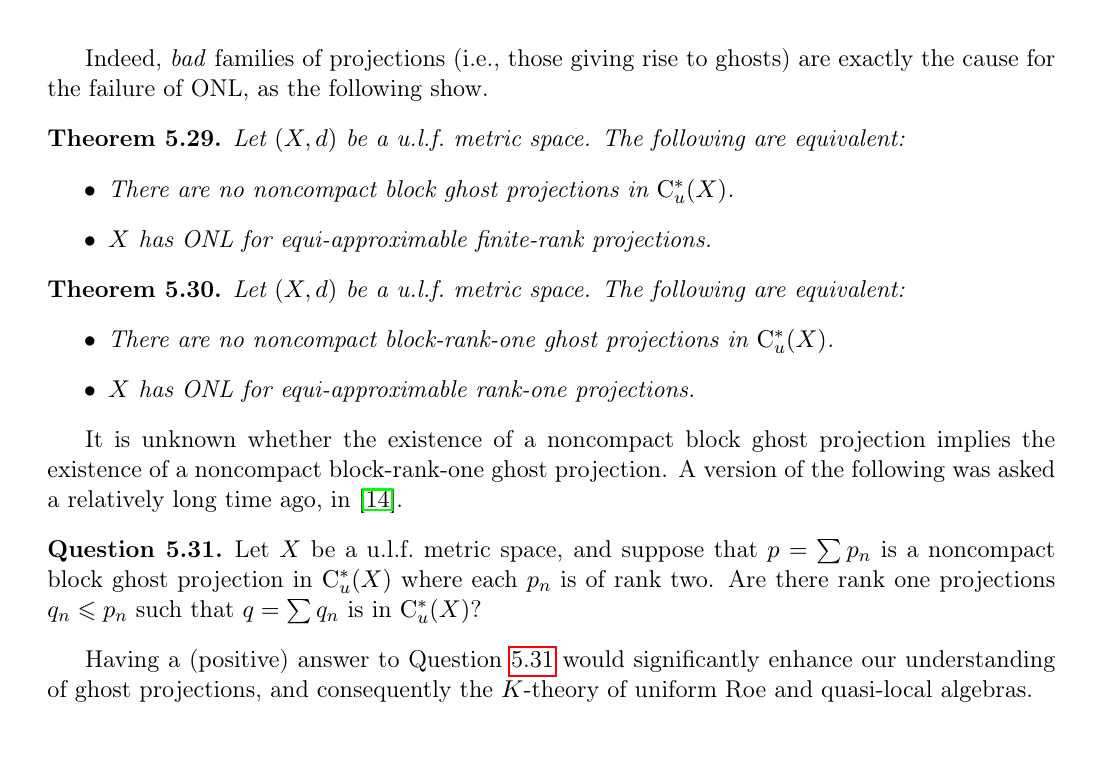
\includegraphics[width=0.94\textwidth]{figures/rank_two_question_crop.png}
\caption{The rank-two block question in the 2026 habilitation.}
\end{figure}
\clearpage
\section{Definitions and scope}
Let $X$ be a uniformly locally finite metric space. A projection
$p\in\Cu(X)$ is a \emph{block projection} if there are pairwise disjoint
finite sets $X_n\subseteq X$ such that
\[
 p=\SOT_{n\in\mathbb N}p_n,\qquad p_n=\chi_{X_n}p\chi_{X_n}.
\]
The $p_n$ are mutually orthogonal finite-rank projections. It is
\emph{block-rank-one} when every nonzero $p_n$ has rank one.
An operator $a\in\Cu(X)$ is a \emph{ghost} if its matrix coefficients
tend to zero at infinity. We use only two elementary facts: diagonal
multipliers $\chi_A$ lie in $\ell_\infty(X)\subseteq\Cu(X)$, and
$\Cu(X)$ is closed under continuous functional calculus.
\section{Proof intuition}
For rank two, some coordinate cut always distinguishes two orthogonal
directions by a fixed amount.  For a fixed higher rank, a compactness
argument on isotropic measures on complex projective space supplies finitely
many diagonal tests, one of which gives a uniformly isolated top eigenvalue
in every block.  Finite thresholding and continuous functional calculus then
extract a rank-one subprojection from every block.

For a non-block Boolean family, an arbitrary finite-rank orthogonal sequence
has a subsequence which is a summable perturbation of projections supported
on pairwise disjoint finite coordinate sets.  Boolean subseries survive that
perturbation.  The block theorem selects rank one, and a compactly perturbed
partial isometry transports the selections back to the original projections.
\section{The diagonal-gap lemma}
\begin{lemma}[uniform two-dimensional coordinate gap]\label{lem:gap}
Let $E$ be a two-dimensional subspace of $\ellTwo(F)$, where $F$ is finite,
and let $P$ be the orthogonal projection onto $E$. There is $A\subseteq F$
such that the two eigenvalues of $(P\chi_A P)|_E$ differ by at least $1/4$.
\end{lemma}
\begin{proof}
Choose an orthonormal basis $u,v$ of $E$. For $x\in F$, put
\[
 d_x=|u(x)|^2-|v(x)|^2,\qquad z_x=\overline{u(x)}v(x).
\]
Then $\sum_xd_x=0$ and $\sum_xz_x=0$. For any $A\subseteq F$, the
eigenvalue gap of $(P\chi_A P)|_E$ is
\begin{equation}\label{eq:gap}
 \left(\left|\sum_{x\in A}d_x\right|^2+
 4\left|\sum_{x\in A}z_x\right|^2\right)^{1/2}.
\end{equation}
Set $D=\sum_x|d_x|$. If $D\geq 1/2$, take
$A=\{x:d_x\geq0\}$. Since $\sum_xd_x=0$,
$\sum_{x\in A}d_x=D/2\geq1/4$, and \eqref{eq:gap} gives the result.
Suppose $D<1/2$. Writing $a_x=|u(x)|^2$ and $b_x=|v(x)|^2$, we have
\[
 2|z_x|=2\sqrt{a_xb_x}\geq a_x+b_x-|a_x-b_x|.
\]
Thus $L:=\sum_x|z_x|>(2-1/2)/2=3/4$. Averaging over
$\theta\in[0,2\pi]$ gives a $\theta$ such that
\[
 \sum_x\left|\operatorname{Re}(e^{-i\theta}z_x)\right|\geq\frac{2L}{\pi}.
\]
Let $A=\{x:\operatorname{Re}(e^{-i\theta}z_x)\geq0\}$. Because
$\sum_xz_x=0$,
\[
 \left|\sum_{x\in A}z_x\right|\geq\frac{L}{\pi}>\frac{3}{4\pi}.
\]
The second term in \eqref{eq:gap} makes the gap larger than
$3/(2\pi)>1/4$.
\end{proof}
\section{Rank-two block selection}
\begin{theorem}\label{thm:main}
Let $X$ be a uniformly locally finite metric space and let
$p\in\Cu(X)$ be a block projection with respect to pairwise disjoint
finite sets $(X_n)_{n\in\mathbb N}$. Suppose every nonzero block
$p_n=\chi_{X_n}p\chi_{X_n}$ has rank two. Then there are rank-one
projections $q_n\leq p_n$ such that
\[
 q=\SOT_{n\in\mathbb N}q_n\in\Cu(X).
\]
In fact, for every $M\subseteq\mathbb N$,
$q_M=\SOT_{n\in M}q_n$ belongs to $\Cu(X)$.
\end{theorem}
\begin{proof}
By Lemma~\ref{lem:gap}, for every $n$ there is $A_n\subseteq X_n$ such
that the two eigenvalues
\[
0\leq\lambda_n^-\leq\lambda_n^+\leq1
\quad\text{of}\quad h_n=(p_n\chi_{A_n}p_n)|_{p_n\ellTwo(X)}
\]
satisfy $\lambda_n^+-\lambda_n^-\geq1/4$.
Let $T=\{k/16:1\leq k\leq15\}$. For every $n$, choose
$t(n)\in T$ so that
\begin{equation}\label{eq:margin}
\lambda_n^-+\frac1{32}\leq t(n)\leq\lambda_n^+-\frac1{32}.
\end{equation}
Such a grid point exists because the interval between the two endpoints has
length at least $3/16$. Put $I_t=\{n:t(n)=t\}$ and $A=\bigcup_nA_n$.
For $I\subseteq\mathbb N$, set
\[
p_I=\SOT_{n\in I}p_n
=\chi_{\bigcup_{n\in I}X_n}p\chi_{\bigcup_{n\in I}X_n}.
\]
Hence $p_I\in\Cu(X)$. For every $t\in T$,
\[
a_t=p_{I_t}\chi_Ap_{I_t}
=\SOT_{n\in I_t}p_n\chi_{A_n}p_n
\]
also belongs to $\Cu(X)$. Choose a continuous function
$f_t:[0,1]\to[0,1]$ that is zero on $[0,t-1/64]$ and one on
$[t+1/64,1]$. The margins in \eqref{eq:margin} imply that
\[
q^{(t)}:=f_t(a_t)
\]
is the block projection whose block in $p_n\ellTwo(X)$, for $n\in I_t$,
is the spectral projection of $h_n$ associated with $\lambda_n^+$.
Thus every nonzero block of $q^{(t)}$ has rank one, and continuous
functional calculus gives $q^{(t)}\in\Cu(X)$.
Since $T$ is finite,
\[
q=\sum_{t\in T}q^{(t)}\in\Cu(X).
\]
Writing $q_n=\chi_{X_n}q\chi_{X_n}$ yields rank-one $q_n\leq p_n$ and
$q=\SOT_nq_n$. Finally, for every $M\subseteq\mathbb N$,
\[
q_M=\chi_{\bigcup_{n\in M}X_n}q\chi_{\bigcup_{n\in M}X_n}\in\Cu(X).
\]
\end{proof}
\section{The bounded-rank block extension}
\begin{lemma}[finitely many coordinate tests in fixed rank]\label{lem:fixedrank}
For every integer $r\geq2$ there are $N_r\in\mathbb N$ and
$\gamma_r>0$ with the following property.  Suppose $(F_n)_n$ are pairwise
disjoint finite sets and $E_n\subseteq\ellTwo(F_n)$ has dimension $r$.
Writing $P_n$ for the projection onto $E_n$, there are diagonal positive
contractions $d_1,\ldots,d_{N_r}$ on $\ellTwo(\bigcup_nF_n)$ such that, for
every $n$, some $(P_nd_jP_n)|_{E_n}$ has a simple largest eigenvalue whose
distance from the second largest eigenvalue is at least $\gamma_r$.
\end{lemma}
\begin{proof}
Identify an $r$-dimensional Hilbert space with $\mathbb C^r$.  Let
$\mathcal K_r$ be the weak-star compact space of positive measures $\mu$ on
complex projective space $\mathbb{CP}^{r-1}$ satisfying
\[
 \int ww^*\,d\mu([w])=I_r.
\]
(The integrand is independent of the unit representative of $[w]$.)
Fix $\mu\in\mathcal K_r$ and $[w_0]\in\operatorname{supp}(\mu)$.  Choose
$0<\varepsilon<1/4$ and a continuous $f:\mathbb{CP}^{r-1}\to[0,1]$,
nonzero in $L_1(\mu)$, supported where
$|\langle w,w_0\rangle|^2>1-\varepsilon$.  Put
\[
 H_f(\mu)=\int f([w])ww^*\,d\mu([w]),\qquad
 m=\int f\,d\mu>0.
\]
The Rayleigh quotient at $w_0$ is at least $(1-\varepsilon)m$.  On
$w_0^\perp$ it is at most $\varepsilon m$, so the min--max principle gives
\[
 \lambda_1(H_f(\mu))-\lambda_2(H_f(\mu))
 \geq(1-2\varepsilon)m>0.
\]
The same strict inequality, with a smaller positive margin, holds on a
weak-star neighborhood of $\mu$.  Compactness of $\mathcal K_r$ therefore
gives finitely many functions $f_1,\ldots,f_{N_r}$ and a common margin
$\gamma_r>0$.

For each $n$, fix a unitary $U_n:E_n\to\mathbb C^r$ and set
$v_{n,x}=U_nP_n\delta_x$.  The measure
\[
 \mu_n=\sum_{x:v_{n,x}\ne0}\|v_{n,x}\|^2
       \delta_{[v_{n,x}/\|v_{n,x}\|]}
\]
belongs to $\mathcal K_r$.  Because the $F_n$ are disjoint, the prescriptions
\[
 d_j(x)=f_j([v_{n,x}/\|v_{n,x}\|])\quad(x\in F_n, v_{n,x}\ne0)
\]
define global diagonal contractions.  In the basis $U_n$, the compression
$P_nd_jP_n$ is exactly $H_{f_j}(\mu_n)$, proving the claim.
\end{proof}

\begin{theorem}[uniformly bounded-rank block selection]\label{thm:boundedblock}
Let $p\in\Cu(X)$ be a block projection with finite blocks $p_n$ satisfying
$2\leq\operatorname{rank}(p_n)\leq R$.  Then there are rank-one
$q_n\leq p_n$ such that $q_M=\SOT_{n\in M}q_n$ belongs to $\Cu(X)$ for
every $M\subseteq\mathbb N$.
\end{theorem}
\begin{proof}
Partition the blocks according to their rank $r\in\{2,\ldots,R\}$.
For each $r$, apply Lemma~\ref{lem:fixedrank} and stitch its diagonal tests
over the disjoint block supports.  Thus each rank-$r$ block has, for one of
finitely many tests $d_{r,j}$, a top eigenvalue separated from the rest by
$\gamma_r$.

Choose a finite grid $T_r\subset[0,1]$ fine enough that whenever
$\lambda_1-\lambda_2\geq\gamma_r$, some $t\in T_r$ satisfies
\[
 \lambda_2+\gamma_r/4\leq t\leq\lambda_1-\gamma_r/4.
\]
Partition the indices into the finitely many classes determined by
$(r,j,t)$.  If $I$ is one class, then
$p_I=\SOT_{n\in I}p_n$ is a diagonal compression of $p$, hence is in
$\Cu(X)$, and $a_I=p_Id_{r,j}p_I\in\Cu(X)$.  A continuous function which is
zero below $t-\gamma_r/8$ and one above $t+\gamma_r/8$ sends $a_I$ to the
projection onto its blockwise top eigenspaces.  Those eigenspaces are
one-dimensional.  Summing over the finitely many classes gives
$q=\SOT_nq_n\in\Cu(X)$.  Finally, every $q_M$ is a diagonal compression of
the block projection $q$.
\end{proof}

\begin{corollary}\label{cor:ghost}
Every noncompact block ghost projection in $\Cu(X)$ whose nonzero blocks
have uniformly bounded finite rank contains a noncompact block-rank-one
ghost projection.  Consequently, Question~5.31 of \cite{Vig} has an
affirmative answer.
\end{corollary}
\begin{proof}
Apply Theorem~\ref{thm:boundedblock}. The resulting $q$ has infinite rank and is
therefore noncompact. Since $0\leq q\leq p$, for every $x,y\in X$,
\[
|\langle q\delta_y,\delta_x\rangle|^2
\leq\langle q\delta_x,\delta_x\rangle\langle q\delta_y,\delta_y\rangle
\leq\langle p\delta_x,\delta_x\rangle\langle p\delta_y,\delta_y\rangle.
\]
The diagonal of the ghost projection $p$ vanishes at infinity, so the
display shows that $q$ is a ghost.
\end{proof}
\section{Arbitrary Boolean families: an infinite subsequence}
\begin{lemma}[disjoint-support gliding hump]\label{lem:glide}
Let $(p_n)_n$ be mutually orthogonal projections of the same finite rank
$r$ on $\ellTwo(X)$.  There are a subsequence $(p_{n_k})_k$, pairwise
disjoint finite sets $F_k\subseteq X$, and rank-$r$ projections
$e_k\in\mathcal B(\ellTwo(F_k))$ such that
\[
 \sum_k\|p_{n_k}-e_k\|<\infty.
\]
\end{lemma}
\begin{proof}
The orthogonality implies $p_n\to0$ strongly.  Hence, for every finite
$F\subseteq X$, $\|p_n\chi_F\|\to0$: strong convergence is uniform on the
finite-dimensional unit ball of $\ellTwo(F)$.

Inductively, after $F_1,\ldots,F_{k-1}$ have been chosen, choose an unused
$n_k$ for which $p_{n_k}$ is as small as desired on their union.  Since
$p_{n_k}$ has finite rank, it is also as small as desired off some finite
set $G_k$ containing that union.  Therefore the compression of $p_{n_k}$
to $F_k=G_k\setminus\bigcup_{i<k}F_i$ is arbitrarily close to $p_{n_k}$.
The spectral projection of this compression for $[1/2,1]$ has rank $r$ and
can be made within $2^{-k}$ of $p_{n_k}$.  Calling it $e_k$ proves the
summability assertion.
\end{proof}

\begin{theorem}[bounded-rank subsequence selection]\label{thm:subsequence}
Let $(p_n)_n$ satisfy the hypotheses of Question~6.1.  Suppose some finite
rank $r\geq2$ occurs for infinitely many $p_n$.  Then there are an infinite
$M\subseteq\mathbb N$ and rank-one $q_n\leq p_n$ for $n\in M$ such that
$\SOT_{n\in M_0}q_n\in\Cu(X)$ for every $M_0\subseteq M$.
In particular, Question~6.1(2) has an affirmative answer whenever the ranks
are uniformly bounded, and for every arbitrary-support rank-two family.
\end{theorem}
\begin{proof}
Restrict to the infinite constant-rank subfamily and apply
Lemma~\ref{lem:glide}; relabel it as $(p_k)_k$, with block projections
$(e_k)_k$.  For every $M\subseteq\mathbb N$, the series
\[
 e_M-p_M=\sum_{k\in M}(e_k-p_k)
\]
converges absolutely in norm.  It is compact, so $e_M\in\Cu(X)$.  In
particular $e=\SOT_ke_k$ is a rank-$r$ block projection in $\Cu(X)$.
Theorem~\ref{thm:boundedblock} gives rank-one $s_k\leq e_k$ with every
$s_M\in\Cu(X)$.

For each $k$, let $v_k$ be the canonical partial isometry from
$e_k\ellTwo(X)$ onto $p_k\ellTwo(X)$ obtained from the polar decomposition
of $p_ke_k$.  By making the errors in Lemma~\ref{lem:glide} still smaller,
the standard close-projections estimate gives
$\sum_k\|v_k-e_k\|<\infty$.  The initial projections of the $v_k$ are
orthogonal, as are their final projections, so $v=\SOT_kv_k$ is a partial
isometry.  Moreover $v-e$ is an absolutely norm-convergent series of
finite-rank operators; hence $v\in\Cu(X)$.  Put
$q_k=v_ks_kv_k^*$.  Then $q_k\leq p_k$ has rank one, and for every $M$,
\[
 \SOT_{k\in M}q_k=vs_Mv^*\in\Cu(X).
\]
\end{proof}
\section{Verification, limitations, and novelty}
The script \texttt{code/verify\_rank\_two\_gap.py} numerically enumerates
all coordinate subsets for random finite rank-two subspaces and checks the
$1/4$ gap bound. This is only a consistency check; Lemma~\ref{lem:gap} is
the proof.
The results do not settle Question~6.1 when the ranks tend to infinity or
are infinite, and they do not give the all-indices conclusion for arbitrary
non-block families.  They do remove the complete bounded-rank block
obstruction and settle the infinite-subsequence part whenever a finite rank
occurs infinitely often.
A bounded search on 22 July 2026 covered arXiv, the published EMS version,
exact phrases from Question~6.1, combinations of uniform Roe, rank two, and
rank-one subprojection, and Vignati's January 2026 habilitation. No prior proof
of these selection statements was found; the habilitation still labels the
rank-two block case Question~5.31. This is not an exhaustive novelty claim.
Human review should focus on the projective-measure compactness lemma, the
finite-threshold functional calculus, and the summable-perturbation transfer.
\begin{thebibliography}{9}
\bibitem{BFV}
B. M. Braga, I. Farah, and A. Vignati,
\emph{Operator norm localization property for equi-approximable families
of projections}, J. Noncommut. Geom. 18 (2024), no. 2, 657--680;
arXiv:2211.02775, DOI:
\href{https://doi.org/10.4171/JNCG/555}{10.4171/JNCG/555}.
\bibitem{Vig}
A. Vignati, \emph{Rigidity of Roe-like algebras},
M\'emoire d'habilitation \`a diriger des recherches, 2026,
Question~5.31, p.~53.
\end{thebibliography}
\end{document}
